\documentclass{ximera}

\input{../../preamble.tex}

\author{Jim Talamo and Alex Beckwith}
\license{Creative Commons 3.0 By-NC}


\outcome{Set up and evaluate an integral that gives the length of a curve segment.}

\begin{document}
\begin{exercise}

A cylindrical tank has base radius 5m and height 20m. Suppose the tank is filled to a height $h$ with mercury ($\rho_{\text{Hg}}$=13593 kg/m$^3$), and then filled the rest of the way with water ($\rho_{\text{H$_2$O}}$=1000 kg/m$^3$). Assume the liquids do not mix. 

Denote the work required to pump the liquids out of the tank (again, when the tank is filled with mercury to height $h$) by $W_{\text{Hg}}(h)$ and $W_{\text{H$_2$O}}(h)$, respectively.

\begin{image}
	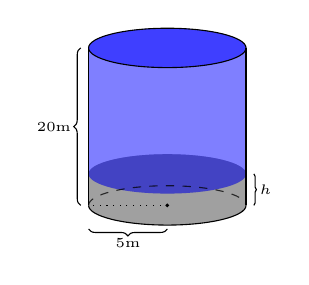
\begin{tikzpicture}
	
	\fill [gray,opacity=0.75] (0,-1.6) ellipse (1 and 0.25);
	\fill [gray,opacity=0.75] (-1,-1.6) -- (-1,-2) arc (180:360:1 and 0.25) -- (1,-1.6) arc (0:180:1 and 0.25);
	
	\fill [blue,opacity=0.5] (0,0) ellipse (1 and 0.25);
	\fill [blue,opacity=0.5] (-1,0) -- (-1,-1.6) arc (180:360:1 and 0.25) -- (1,0) arc (0:180:1 and 0.25);
	
	\draw (0,0) ellipse (1 and 0.25);
	\draw (-1,0) -- (-1,-2);
	\draw (-1,-2) arc (180:360:1 and 0.25);
	\draw [dashed,opacity=0.75] (-1,-2) arc (180:360:1 and -0.25);
	\draw (1,-2) -- (1,0);  
	
	\node[circle,fill,inner sep=0.5pt] at (0,-2) {};
	\draw[dotted] (0,-2) -- (-1,-2);
	
	\draw[decoration={brace,raise=.1cm},decorate,thin] (-1,-2) -- (-1,0);
	\node[anchor=east] at (-1.1,-1) {\tiny $20$m};
	
	\draw[decoration={brace,raise=.1cm,amplitude=+0.9pt},decorate,thin] (1,-1.6) -- (1,-2);
	\node[anchor=west] at (1.05,-1.8) {\tiny $h$};
	
	\draw[decoration={brace,raise=.1cm},decorate,thin] (0,-2.2) -- (-1,-2.2);
	\node[anchor=north] at (-0.5,-2.3) {\tiny $5$m};

	\end{tikzpicture}
\end{image}

Compute $W_{\text{Hg}}(10)$, the work required to pump the mercury out of the tank when $h=10$.
\[
W_{\text{Hg}}(10) 
	= \int_{y=\answer{0}}^{y=\answer{10}} \rho_{\text{Hg}} g \answer{25 \pi (20-y)} \d y = \answer[tolerance=10]{499542750 \pi }J
\]

Compute $W_{\text{H$_2$O}}\left(\frac{1}{2}\right)$, the work required to pump the water out of the tank when $h= \frac{1}{2}$.
\[
W_{\text{H$_2$O}}\left(\frac{1}{2}\right) 
	= \int_{y=\answer{\frac{1}{2}}}^{y=\answer{20}} \rho_{\text{H$_2$O}} g \answer{25\pi (20-y)} \d y = \answer[tolerance=10]{46580625 \pi}J
\]

Find a value for $h$ so that the work required to pump the mercury from the tank is equal to the work required to pump the water from the tank.  Express your final answer to 2 decimal places.
\[
h=\answer[tolerance=.01]{20 \left(\frac{14593 - \sqrt{198362649}}{14593} \right)} \text{m}
\]
\end{exercise}
\end{document}
